% Preamble
\documentclass[10pt]{ltjsarticle}

% Packages
\usepackage{amsmath}
\usepackage{mathtools}
% \usepackage[backend=biber,sorting=none]{biblatex}
\usepackage{graphicx}
\usepackage{booktabs}
\usepackage{siunitx}
\usepackage{bm}
\usepackage{physics}

\mathtoolsset{showonlyrefs} % 参照した式のみ番号を表示

\date{}

\begin{document}

\begin{figure}[hbt]
  \centering
  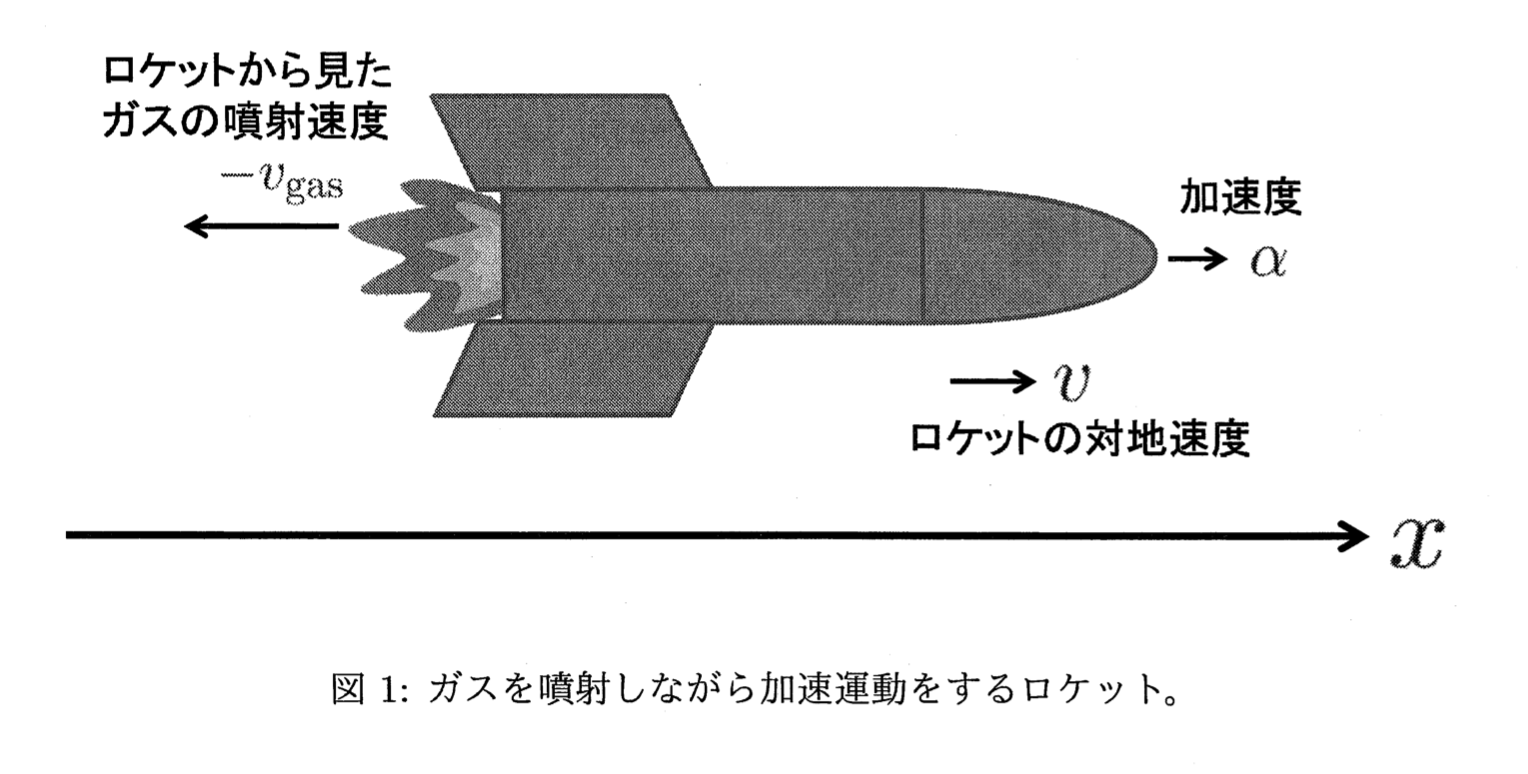
\includegraphics[width=0.6\linewidth,keepaspectratio]{./img/tokyoH28.png}
  % \caption{}
  \label{fig:rocket}
\end{figure}

  ロケットの質量$m$を非相対論的に座標時間$t$の関数として、および相対論的に固有時間$\tau$の関数として表した式を比較して意味を論じる問題。$m$の表式は次のようになる。
  \begin{itemize}
    \item 非相対論的: $m(t) = m_0 e^{-\frac{\alpha}{v_{gas}} t}$
    \item 相対論的: $m'(\tau) = m_0 e^{-\frac{\alpha}{v_{gas}} \tau}$
  \end{itemize}
  回答例としては、ロケットからこの系を見た時、実際の速度は光速度で頭打ちになるが、いつまでも一定加速度$\alpha$で加速し続けているように見えることを意味する、ということらしい。

  \begin{equation}
    t = \frac{\tau}{\sqrt[]{1 - \frac{v^2}{c^2}}}
  \end{equation}
  なので、ローレンツ因子$\dfrac{1}{\sqrt{1 - \frac{v^2}{c^2}}}$の分変わってくるのはわかるが、解釈の仕方が今ひとつわからない、

  $t > \tau$だから、$m < m'$で、運動している物体の質量は静止質量よりも大きいね、ということかと思ったけど、違うのかな$\cdots$?
\end{document}